\section{Results}
\label{sec4}
In this section, we present and analyze the obtained results regarding the execution of the planners on 
the PDDL files.

The submitted archive contains the solutions to the presented problems and it is organized as follows.
We have created four folders, one for each problem, that contain the PDDL domain files and one or more 
PDDL problem files. For each problem file, the plan found by the planner is reported in a separate file.
For Problem 4, there is a folder that contains all the code required to execute the \texttt{PlanSys2} 
problem.
% For each problem there is a folder that contains the PDDL domain file and one or more PDDL problem files.
% the plan obtained running the planner on each problem file is reported in 


\subsection{Problem 1}
For this problem, we have modeled two PDDL problem files with increasing complexity.
The planner used to found the solution is \texttt{Downward} using the option \texttt{--alias lama-first}.

In the first problem modeled, there are 4 people, 5 crates, 4 locations and the planner successfully
found an optimal solution that requires the execution of 15 actions.

The second problem modeled is a bit more complex: the number of objects modeled increase to 8 people, 
8 crates and 5 locations. Also in this case, the planner successfully
found an optimal solution that requires the execution of 27 actions.


\subsection{Problem 2}
For this problem, the planner used is \texttt{Enhsp-2020} that is available in \texttt{Planutils}.

The modeled PDDL problem contains 6 people, 6 crates, 4 locations and just one carrier with capacity 4.
Executing the planner with the option \texttt{-anytime}, it managed to find an optimal solution that 
requires performing 16 actions.

\subsection{Problem 3}
For this problem, the planner used is \texttt{Optic} that is available in \texttt{Planutils}.

It has been decided to model two PDDL problem files.
In the second one, there are two robots and two carriers while in the first one only one of both.
In this way, as previously explained, only in the second problem the actions can be perfomed in parallel.

The planner managed to find a plan of duration 34 seconds for for the first problem and a plan of
duration 24 seconds for the second one.
As can be seen in the second plan, some actions are performed simultaneously as desired.

\subsection{Problem 4}
For this problem, the PDDL domain and problem are the same of Problem 3.
The problem is specified using a list of terminal commands accepted by \texttt{PlanSys2}.
These commands are reported in a file located in the directory of Problem 4.
% The terminal commands required to specify the problem are the equivalent of the PDDL problem file of the 
% Problem 3 and are reported in the directory of Problem 4. TODO


\begin{figure}[t]
\centerline{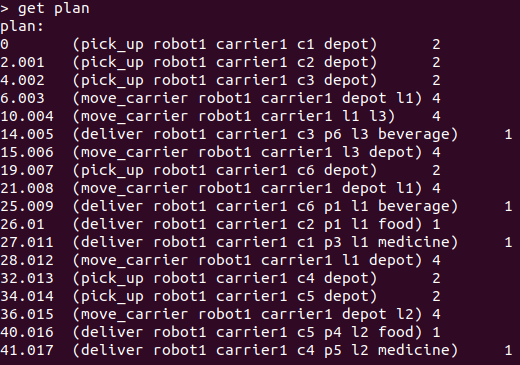
\includegraphics[scale=0.45]{assignment_terminal.png}}
\caption{Plan found by \texttt{POPF} planner.}
\label{fig:plan}
\end{figure}
    
\begin{figure}[t]
\centerline{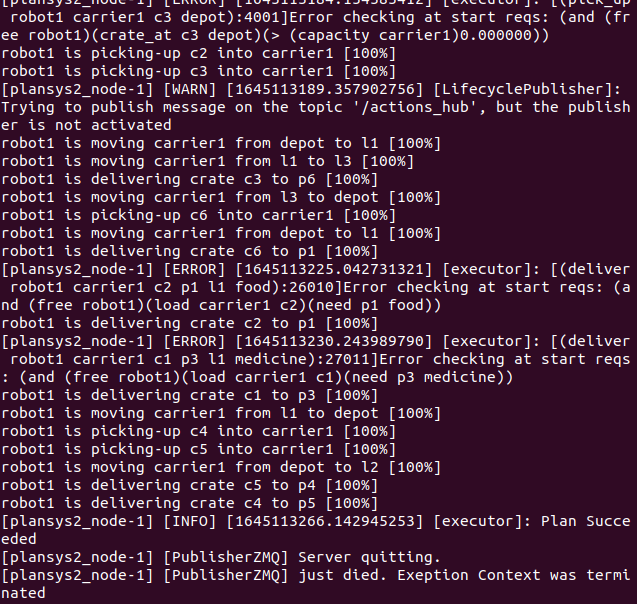
\includegraphics[scale=0.365]{assignment_run.png}}
\caption{\texttt{PlanSys2} execution of the plan.}
\label{fig:execution}
\end{figure}

Executing the \texttt{POPF} planner on this problem, it managed to find the plan shown in Figure 
\ref{fig:plan} of duration 42 seconds.
This plan is then executed by \texttt{PlanSys2} within the \texttt{ROS2} framework. 
Figure \ref{fig:execution} shows part of the execution of the plan and the messages sended by the action nodes.
